\documentclass[11pt, handout]{beamer}

\usepackage[utf8]{inputenc}
\usepackage[francais]{babel}
\usepackage{tcolorbox}
\usepackage{minted}
\usepackage{pdfpages}
\usepackage{sourcecodepro}
\usepackage{graphicx}

\graphicspath{{img/}}

% Scala
\newminted{scala}{frame=single, framesep=6pt, breaklines=true,
  fontsize=\scriptsize,autogobble}
\newmintedfile{scala}{frame=single, framesep=6pt, breaklines=true,
  fontsize=\scriptsize,autogobble}

% VHDL
\newminted{vhdl}{frame=single,framesep=6pt, breaklines=true,
  fontsize=\scriptsize,autogobble}
\newmintedfile{vhdl}{frame=single, framesep=6pt, breaklines=true,
  fontsize=\scriptsize,autogobble}

% JavaScript
\newminted{javascript}{frame=single,framesep=6pt, breaklines=true,
  fontsize=\scriptsize,autogobble}
\newmintedfile{javascript}{frame=single, framesep=6pt, breaklines=true,
  fontsize=\scriptsize,autogobble}

% DOT
\newminted{text}{frame=single,framesep=6pt, breaklines=true,
  fontsize=\scriptsize,autogobble}

\usetheme{CambridgeUS}
\setbeamertemplate{\insertframenumber/\inserttotalframenumber}

\title[KlugHDL]{KlugHDL : a SpinalHDL diagram generator}
\subtitle[PA]{Défense de projet d'approfondissement}
\author{Sylvain Julmy}
\institute[MSE]{Institut Systèmes Industriels\\Master of Science HES-SO}
\date{\today}

\AtBeginSection[]{
  \begin{frame}
    \frametitle{Schedule}
    \tableofcontents[
    currentsubsection,
    sectionstyle=show/shaded,
    ]
  \end{frame}
}

\begin{document}

\maketitle

\begin{frame}
  \frametitle{Overview of contents}
    \tableofcontents[]
\end{frame}

\section{Context}


\begin{frame}
  \frametitle{VHDL}
  \begin{itemize}
  \item Hardware description language
  \item Mostly use with Verilog for programming on the FPGA
  \item Old, verbose and tricky
  \end{itemize}
\end{frame}

\begin{frame}
  \frametitle{SpinalHDL}

  \begin{tcolorbox}
  SpinalHDL, written as an internal DSL, is used to describe digital hardware and generate the corresponding
  source code in VHDL (or Verilog).
  \end{tcolorbox}

\end{frame}

\begin{frame}[fragile]
  \frametitle{VHDL vs SpinalHDL}

  \begin{minipage}{0.45\textwidth}
  \begin{scalacode}
  import spinal.core._
  
  class AND extends Component {
    val io = new Bundle {
      val a = in Bool
      val b = in Bool
      val c = out Bool
    }
    io.c := io.a & io.b
  }
  \end{scalacode}
  \end{minipage}
  \hfill
  \begin{minipage}{0.45\textwidth}
  \begin{vhdlcode}
  entity AND_1 is
    port(
      io_a : in std_logic;
      io_b : in std_logic;
      io_c : out std_logic
    );
  end AND_1;
   
  architecture arch of AND_1 is
  begin
    io_c <= (io_a and io_b);
  end arch;
  \end{vhdlcode}
  \end{minipage}
\end{frame}

\begin{frame}
  \frametitle{KlugHDL}
  \begin{tcolorbox}
  An application which is able to analyse a SpinalHDL program and produce a
  block diagram of the corresponding hardware description.
  \end{tcolorbox}
\end{frame}

\begin{frame}
  \frametitle{KlugHDL}
  \begin{center}
  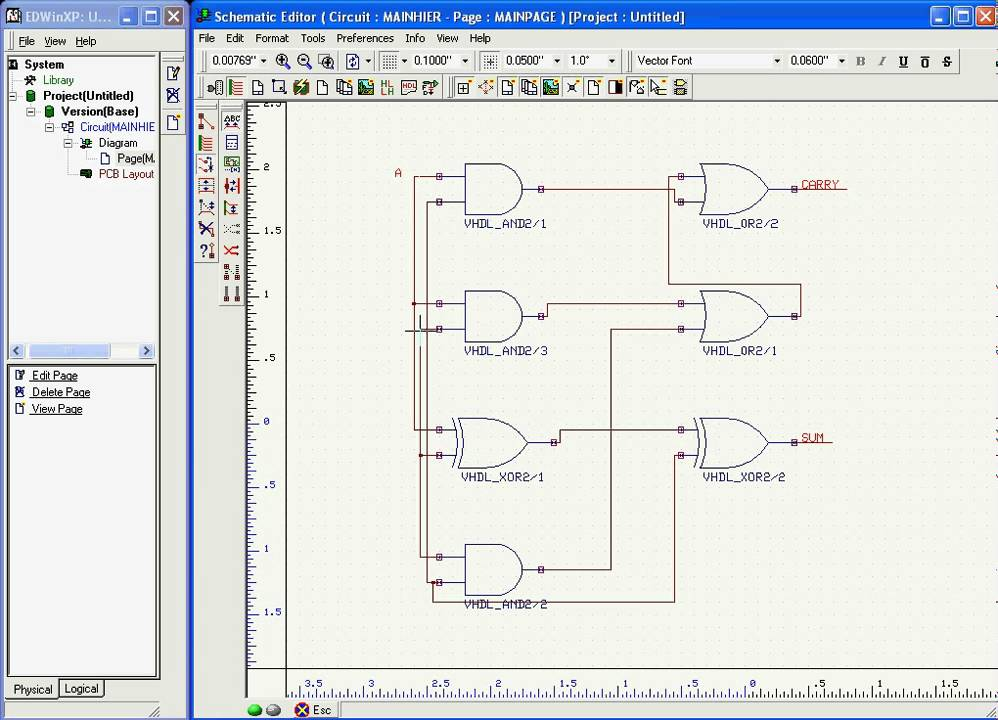
\includegraphics[width=0.8\textwidth]{vhdl_diagram_example}
  \end{center}
\end{frame}

\section{Diagrams modelling}

\begin{frame}
  \frametitle{Architecture}
  \begin{center}
    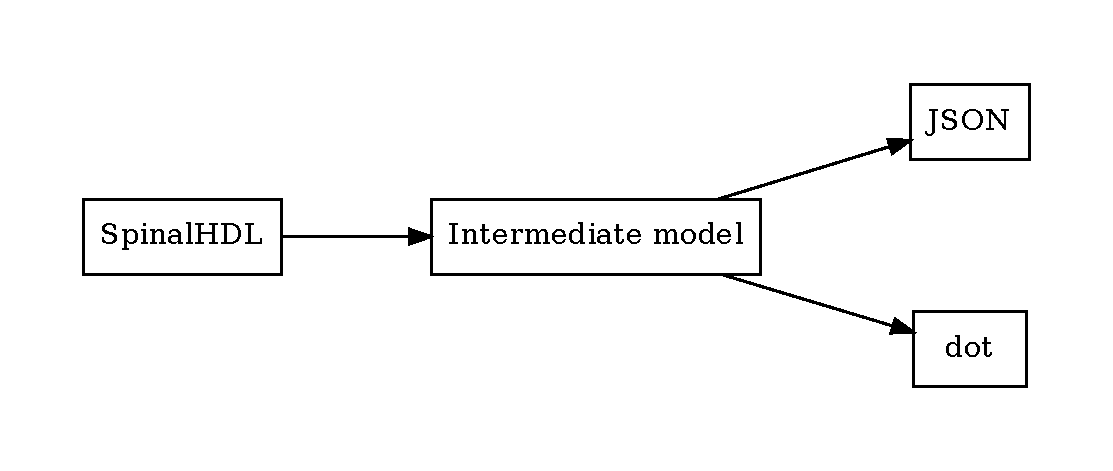
\includegraphics[width=0.8\textwidth]{architecture}
  \end{center}
\end{frame}

\begin{frame}
  \frametitle{Visual representation}
  \begin{itemize}
  \item Hierarchical layout
  \item Tree view
  \item Multiple diagrams
  \end{itemize}
\end{frame}

\begin{frame}
  \frametitle{Hierarchical layout}
  \begin{center}
    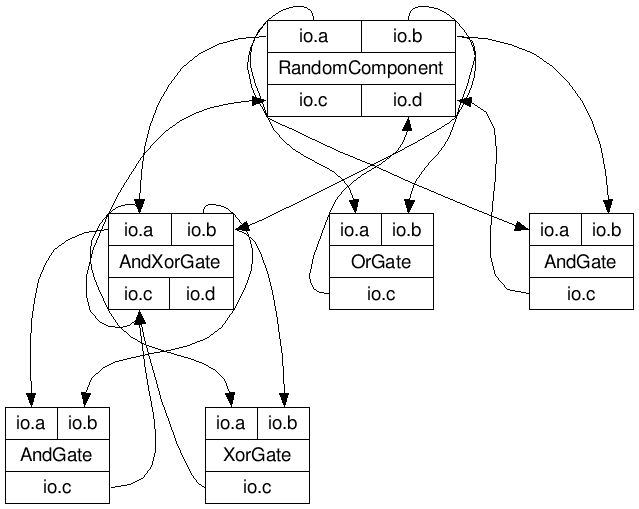
\includegraphics[width=0.7\textwidth]{hierarchical_layout}
  \end{center}
\end{frame}

\begin{frame}
  \frametitle{Tree view}
  \begin{center}
    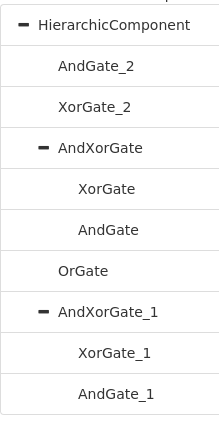
\includegraphics[width=0.3\textwidth]{tree_view}
  \end{center}
\end{frame}

\begin{frame}
  \frametitle{Multiple diagrams}
  \begin{minipage}{0.30\textwidth}
    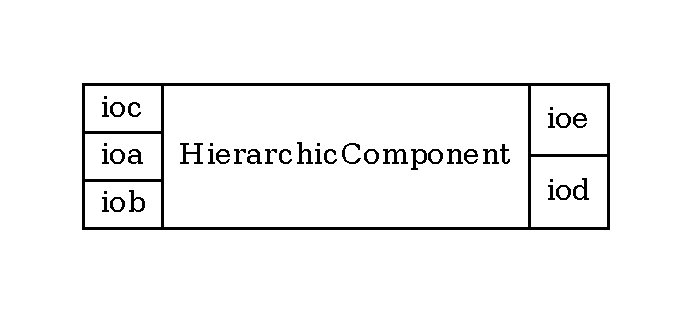
\includegraphics[width=1.0\textwidth]{hierarchic_component}
  \end{minipage}
  \hfill
  \begin{minipage}{0.69\textwidth}
    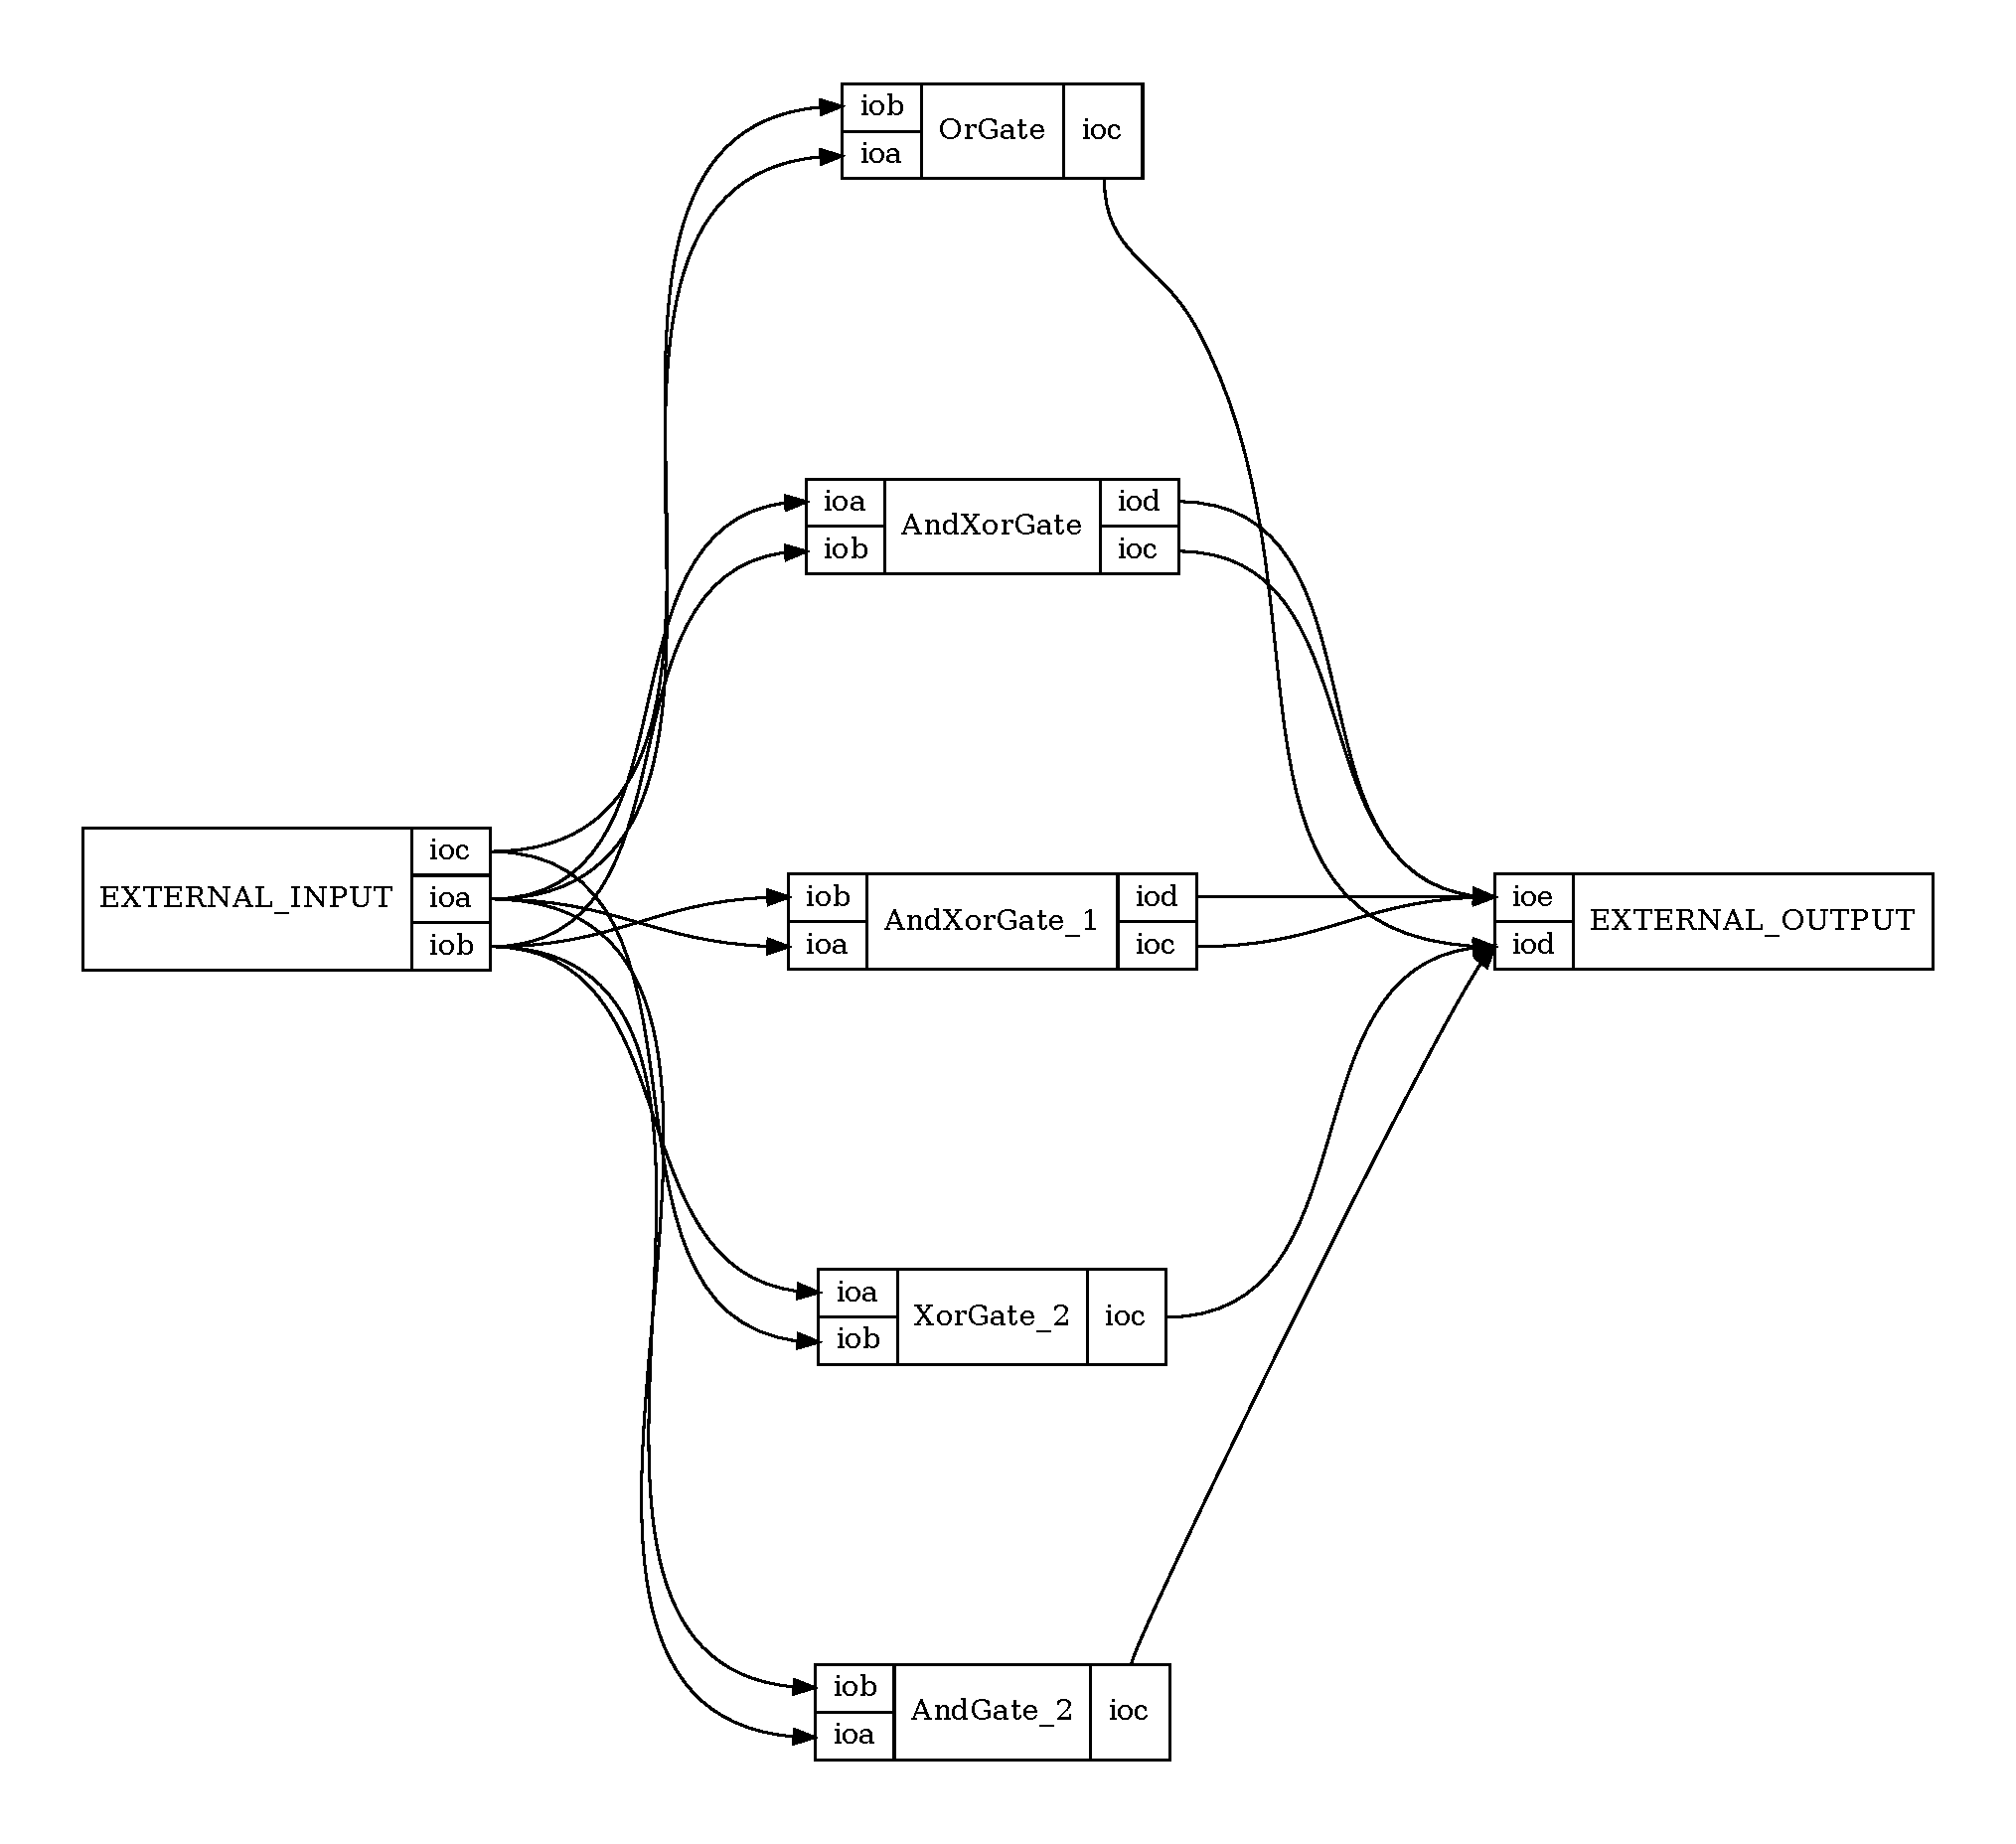
\includegraphics[width=1.0\textwidth]{hierarchic_component_inside}
  \end{minipage}
\end{frame}

\begin{frame}
  \frametitle{Model representation}
  \begin{itemize}
  \item Model owns at least one diagram
  \item Diagram owns one or more component
  \item Component owns some ports
  \item Connections are between ports
  \end{itemize}
\end{frame}

\begin{frame}
  \frametitle{Model representation}
  \begin{center}
    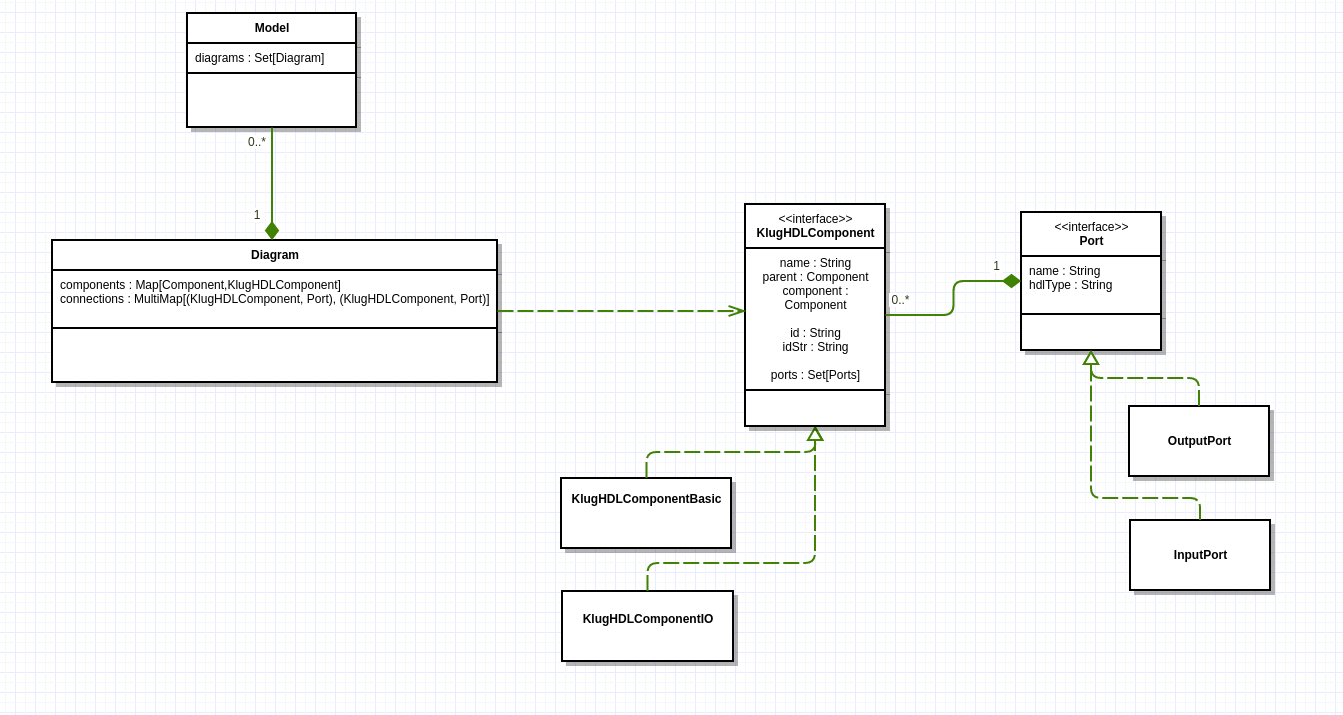
\includegraphics[width=0.8\textwidth]{class-diagram-intermeditate-model}
  \end{center}
\end{frame}

\section{Parsing the AST}

\begin{frame}
  \frametitle{AST}
  \begin{tcolorbox}
  AST : Abstract Syntax Tree
  \end{tcolorbox}
\end{frame}

\begin{frame}
  \frametitle{AST}
  \framesubtitle{Example : $5 * (2 + 3)$}
  \begin{center}
    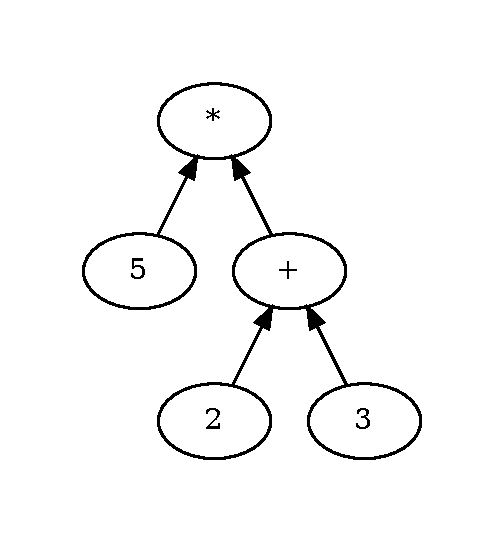
\includegraphics[width=0.5\textwidth]{ast_example}
  \end{center}
\end{frame}

\begin{frame}
  \frametitle{Process}
  \begin{itemize}
  \item Diagram parsing
  \item Component parsing and generation
  \item Ports parsing
  \item Connections parsing
  \end{itemize}
\end{frame}

\section{Viewing library}

\begin{frame}
  \frametitle{Base graph model}
  \begin{center}
    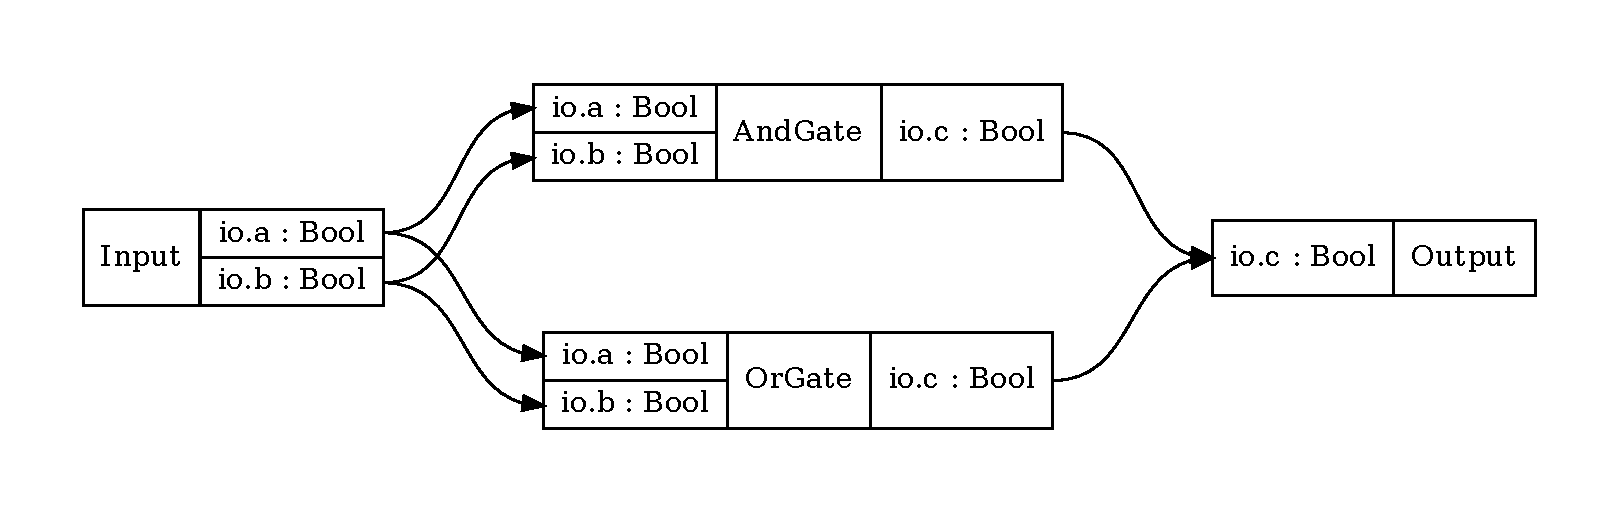
\includegraphics[width=0.9\textwidth]{base_graph_model}
  \end{center}
\end{frame}

\begin{frame}
  \frametitle{GraphStream}
  \begin{tcolorbox}
    GraphStream is a Java library used for the modelling and analysis of dynamic graphs.
  \end{tcolorbox}
\end{frame}

\begin{frame}
  \frametitle{GraphStream}
  \framesubtitle{Implementation of the base graph model}
  \begin{center}
    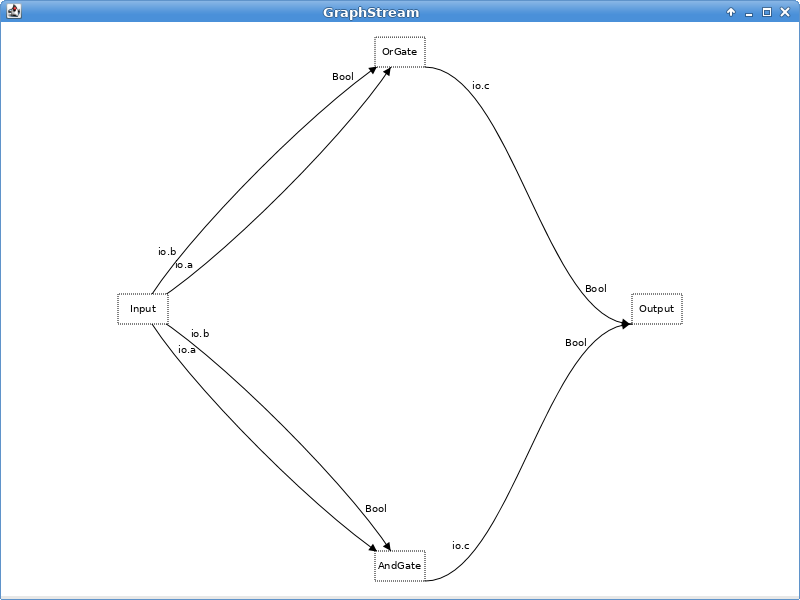
\includegraphics[width=0.8\textwidth]{graphstream_base_model}
  \end{center}
\end{frame}

\begin{frame}
  \frametitle{GraphStream}
  \framesubtitle{Problems}
  \begin{center}
    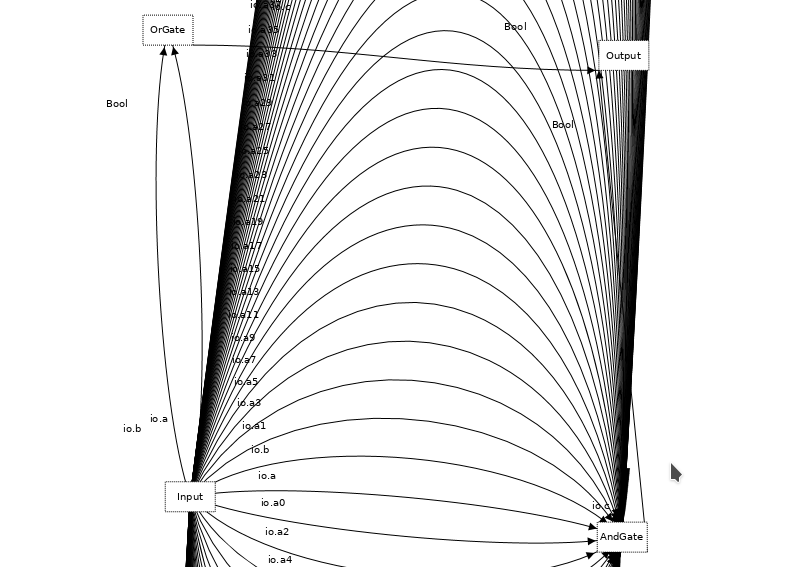
\includegraphics[width=0.8\textwidth]{graphstream_lot_of_edges}
  \end{center}
\end{frame}

\begin{frame}
  \frametitle{GraphStream}
  \framesubtitle{Problems}
  \begin{itemize}
    \item No port notion
    \item Label on the edges
    \item Tricky connection's position
  \end{itemize}
\end{frame}

\begin{frame}
  \frametitle{Draw2D}
  \begin{tcolorbox}
    Draw2D is a HTML5 and Javascript library for visualisation and interaction
    with diagrams and graphs.
  \end{tcolorbox}
\end{frame}

\begin{frame}
  \frametitle{Draw2D}
  \framesubtitle{Implementation of the base graph model}
  \begin{center}
    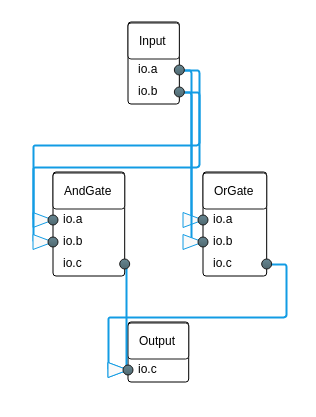
\includegraphics[width=0.45\textwidth]{draw2d_base_model}
  \end{center}
\end{frame}

\begin{frame}
  \frametitle{Draw2D}
  \framesubtitle{Problems : Layout}
  \begin{center}
    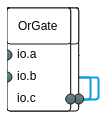
\includegraphics[width=0.3\textwidth]{overlap_draw2d}
  \end{center}
\end{frame}

\begin{frame}
  \frametitle{Draw2D}
  \framesubtitle{Problems : Layout}
  Solutions :
  \begin{itemize}
  \item Implements our owns layout algorithm (for nodes with ports)
  \item Use the layout engine of another program (DOT,...)
  \item Use another library, which might be non-free
  \end{itemize}
\end{frame}

\begin{frame}
  \frametitle{Draw2D}
  \framesubtitle{Problems : Layout}
  \begin{tcolorbox}[colframe=red!75!black]
    We can't (easily) manipulate the vertex layout with Draw2D.
  \end{tcolorbox}
\end{frame}

\section{Diagram visualisation}

\begin{frame}
  \frametitle{Recall}
  \begin{center}
    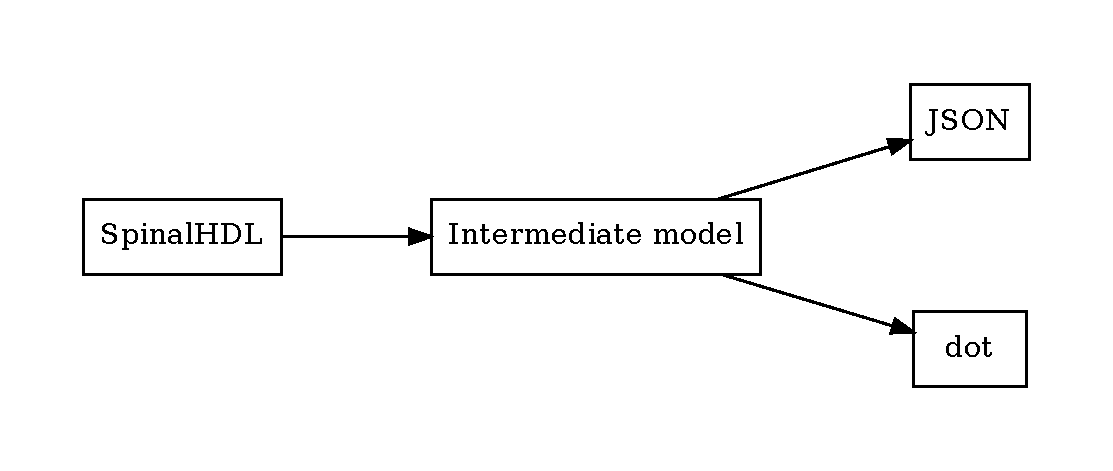
\includegraphics[width=0.8\textwidth]{architecture}
  \end{center}
\end{frame}

\begin{frame}
  \frametitle{DOT}
  \begin{center}
    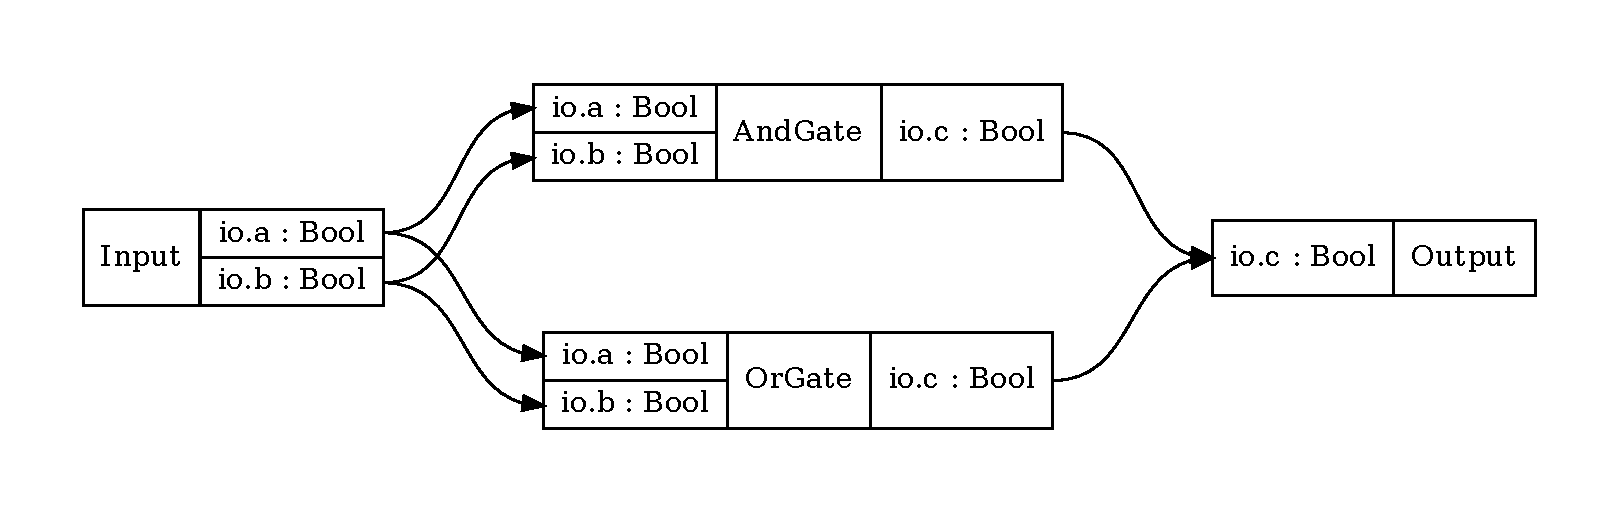
\includegraphics[width=0.9\textwidth]{base_graph_model}
  \end{center}
\end{frame}

\begin{frame}[fragile]
  \frametitle{DOT}
  \begin{center}
    \begin{textcode}
    digraph g {
      node [shape=record];
      graph [rankdir=LR,ranksep="1",nodesep="1"];
      AndGate [label="{{<a>io.a : Bool|<b>io.b : Bool}|AndGate|{<c>io.c : Bool}}"];
      OrGate [label="{{<a>io.a : Bool|<b>io.b : Bool}|OrGate|{<c>io.c : Bool}}"];
      Input [label="{Input|{<a>io.a : Bool|<b>io.b : Bool}}"];
      Output [label="{{<c>io.c : Bool}|Output}"];
      Input:a -> AndGate:a;
      Input:b -> AndGate:b;
      Input:a -> OrGate:a;
      Input:b -> OrGate:b;
      OrGate:c -> Output:c;
      AndGate:c -> Output:c;
    }
    \end{textcode}
  \end{center}
\end{frame}

\begin{frame}
  \frametitle{JSON}
  \begin{tcolorbox}
    JSON (JavaScript Object Notation) is a format mostly used by Javascript for object serialisation.
  \end{tcolorbox}
\end{frame}

\begin{frame}[fragile]
  \frametitle{JSON}
  \begin{center}
    \begin{javascriptcode}
    {
      "tree":{
        "text":"SmallComponent",
        "nodes":[{
          "text":"AndGate"
        },{
          "text":"OrGate"
        }]
      },
      "model":[{
        "diagram":{
          "name":"null",
          "isTopLevel":"true",
          "components":[{
            "name":"SmallComponent",
            "type":"default",
            "ports":[{
    ...
    ...
    \end{javascriptcode}
  \end{center}
\end{frame}

\begin{frame}
  \frametitle{JSON}
  \framesubtitle{Advantages}
  \begin{itemize}
  \item Common backend for multiple libraries
  \item JSON is readable by a lot of languages
  \item Human readable
  \end{itemize}
\end{frame}

\section{Current working state}

\begin{frame}
  \frametitle{Current working state}
  \framesubtitle{What is working}
  \begin{itemize}
  \item Parse and generate the IR for simple SpinalHDL component.
  \item Generate DOT and JSON file.
  \item A dynamic visualisation through a browser.
  \end{itemize}
\end{frame}

\begin{frame}
  \frametitle{Current working state}
  \framesubtitle{What isn't working}
  \begin{itemize}
  \item Parse and generate the IR for more complex SpinalHDL component.
  \item Child to parent navigation
  \item Filter with the tree view
  \end{itemize}
\end{frame}

\section{Further work}

\begin{frame}
  \frametitle{Further work}
  \begin{itemize}
  \item Parsing and generating the intermediate model for any kind of SpinalHDL
    component
  \item Finding a way or improve the library to directly manipulate the Draw2D
    layout
  \item Generate the layout information with DOT and Graphviz and add them to
    KlugHDL
  \end{itemize}
\end{frame}

\begin{frame}
  \frametitle{Conclusion}
  \begin{itemize}
  \item Try to offer a tool for SpinalHDL.
  \item Generate static and dynamic diagram from the SpinalHDL AST.
  \item Some works need to be done.
  \end{itemize}
\end{frame}

\begin{frame}
  \frametitle{Questions ?}
  \begin{tcolorbox}
  \begin{center}
    \Huge Thanks !
  \end{center}
  \end{tcolorbox}
\end{frame}

\end{document}

%%% Local Variables:
%%% TeX-command-extra-options: "-shell-escape"
%%% TeX-master: t
%%% End:
